

Four python scripts: GPS2.py, commande.py, testserial.py et ServeurN.py

The code which have been implemented for this part of the project can be sum up with the following picture \ref{fig:SyntheseCodeRegulationRobot}:

\begin{figure}[ht]
\centering
    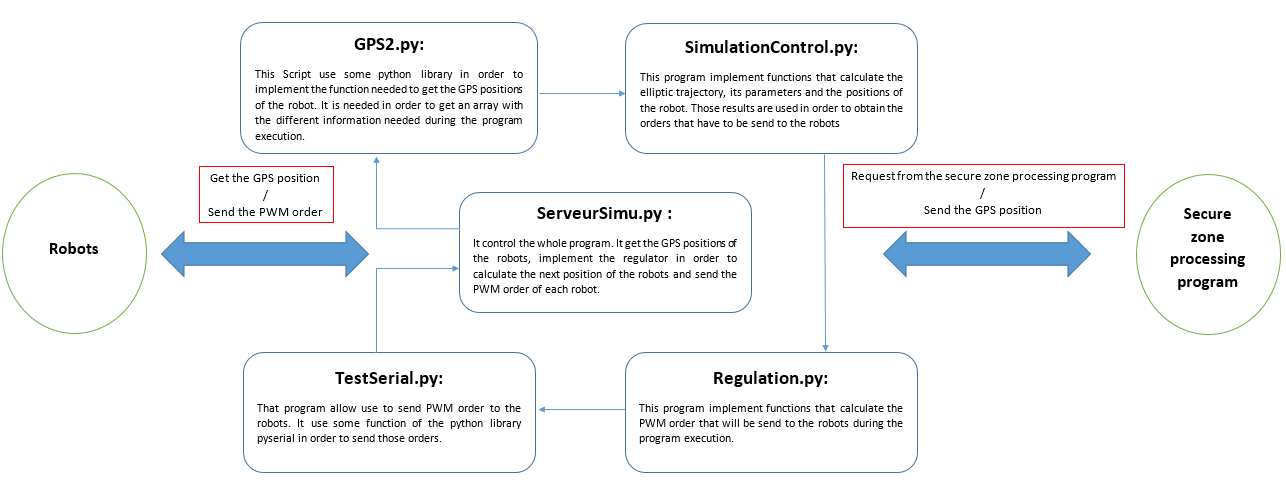
\includegraphics[scale=0.5,angle=90]{SyntheseCodeRegulationRobot.PNG}
    \caption{Architecture of the program which control the regulation of the robots.}
    \label{fig:SyntheseCodeRegulationRobot}
\end{figure}

As you can see, there are 5 main script that are used in order to run the whole program.

\begin{itemize}
\item \textbf{GPS2.py}: this script has been implemented by \textcolor{blue}{\textit{Pierre JACQUOT}} and allow us to get access to the GPS signal of all the robots. This programm catch the first available GPS tram og each robot, put it in a numpy array. The parameters which are keept are the latitude, the longitude, the speed, the north, the east and the time.
\item SimulationControl.py has been implemented by  \textcolor{blue}{\textit{Alice Danckaers}} and is used here in order to get the elliptic trajectory in function of the instant t and the theoretical position of each robots.

\end{itemize}
\pagebreak